\section*{Problem 16}

Consider the system...

$$
\begin{array}{l}
\dot{x}_{1}=-x_{1} \\
\dot{x}_{2}=\left(x_{1} x_{2}-1\right) x_{2}^{3}+\left(x_{1} x_{2}-1+x_{1}^{2}\right) x_{2}
\end{array}
$$


\subsection*{Part A}

By setting the state equations to zero the equilibrium points can be computed as shown below...

$$
\begin{array}{l}
0=-x_{1} \\
0=\left(x_{1} x_{2}-1\right) x_{2}^{3}+\left(x_{1} x_{2}-1+x_{1}^{2}\right) x_{2}
\end{array}
$$

\noindent It is clear that $x_1 =0$ and that by substituting this result into the second state equation, that $x_2 = 0$. Since the system is not valid for any other points which keep the system at equilibrium $x_1=0 \& x_2 =0$ are a \underline{unique equilibrium}.


\subsection*{Part B}

By linearizing the state equations we obtain the following Jacobian Matrix.

$$
A_j =
\begin{bmatrix}
  \frac{\partial f_{1}}{\partial x_{1}} &  \frac{\partial f_{1}}{\partial x_{2}} \\
  \frac{\partial f_{2}}{\partial x_{1}} &  \frac{\partial f_{2}}{\partial x_{2}}
\end{bmatrix}
= \left .
\begin{bmatrix}
  -1 & 0 & \\
  (x_2^4 + x_2^2 + 2x_1x_2) & (4x_1x_2^3-3x_2^2 + 2x_1x_2 -1 x_1^2) &
\end{bmatrix}
\right \rvert_{x_{eq}=0}
$$

\noindent When the Jacobian is evaluated at the equilibrium point $x=0$ it results in the following matrix.

$$
A_j =
\begin{bmatrix}
  -1 & 0 & \\
  0 & -1 &
\end{bmatrix}
$$

\noindent Since $Re(\lambda_i) < 0$, via local analysis, we can show that the sytem is \underline{asympotically stable}.

\subsection*{Part C}

Show that the following set is positively invariant.

$$
\Gamma=\left\{x \in \mathbb{R}^{2} \mid x_{1} x_{2} \geq 2\right\}
$$



\subsubsection*{Solution}
This next problem requires rethinking what it would require for the given set to be \underline{positively invariant}. Unlike previous problems that typically provide an upper bound on the elements of the set, this set places a lower bound on the elements of the set. Since we know that inorder for the system to actually be positively invariant, any trajectory starting in $\Gamma$ must stay in $\Gamma$ for all $t\geq 0$. Since the set is not defined at the equilibrium point which is the origin, we can reason that we \underline{do not want} the system to converge towards the origin as that would violate the definition of the set which is assumed to be invariant. For this specific case though, we can see that if the trajectory goes to infinity $\forall x \in \R^2$, the value is still maintained in the definition of the invariant set. \\

\noindent In this case then, we wish to drive the system away from the origin, anywhere between $[2, \infty)$. Since this is the goal, we are interested in making sure that the system is \underline{unstable} with respect to the origin of the system. This means that we want to ensure that $\dot{V}(x)>0$ (for all valid point of the set) since this condition is what allows the system to diverge away from any the origin.


To test this mathematically we can define...

$$
V(x) = x_1x_2
$$


$$
\begin{array}{l}
\dot{V}(x) = \dot{x}_1x_2 + \dot{x}_2x_1 \\
\dot{V}(x) = -x_1x_2 + x_1 \left( (x_1x_2 -1)x_2^3 + (x_1x_2 - 1+ x_1^2)x_2 \right) \\
\dot{V}(x) = -x_1x_2 +x_1^2x_2^4 -x_1x_2^3 + x_1^2x_2^2 - x_1x_2 + x_1^3x_2
\end{array}
$$

\noindent After simplification we can show that...


$$
\dot{V}(x) \left. \right\rvert_{x_1,x_2=2} > 0
$$

\noindent Since this shows that the system is \underline{unstable} for $x=2$, we can conclude that the set will not converge towards the origin, and hence will be maintained inside of the set, which is unbounded.


\begin{center}
  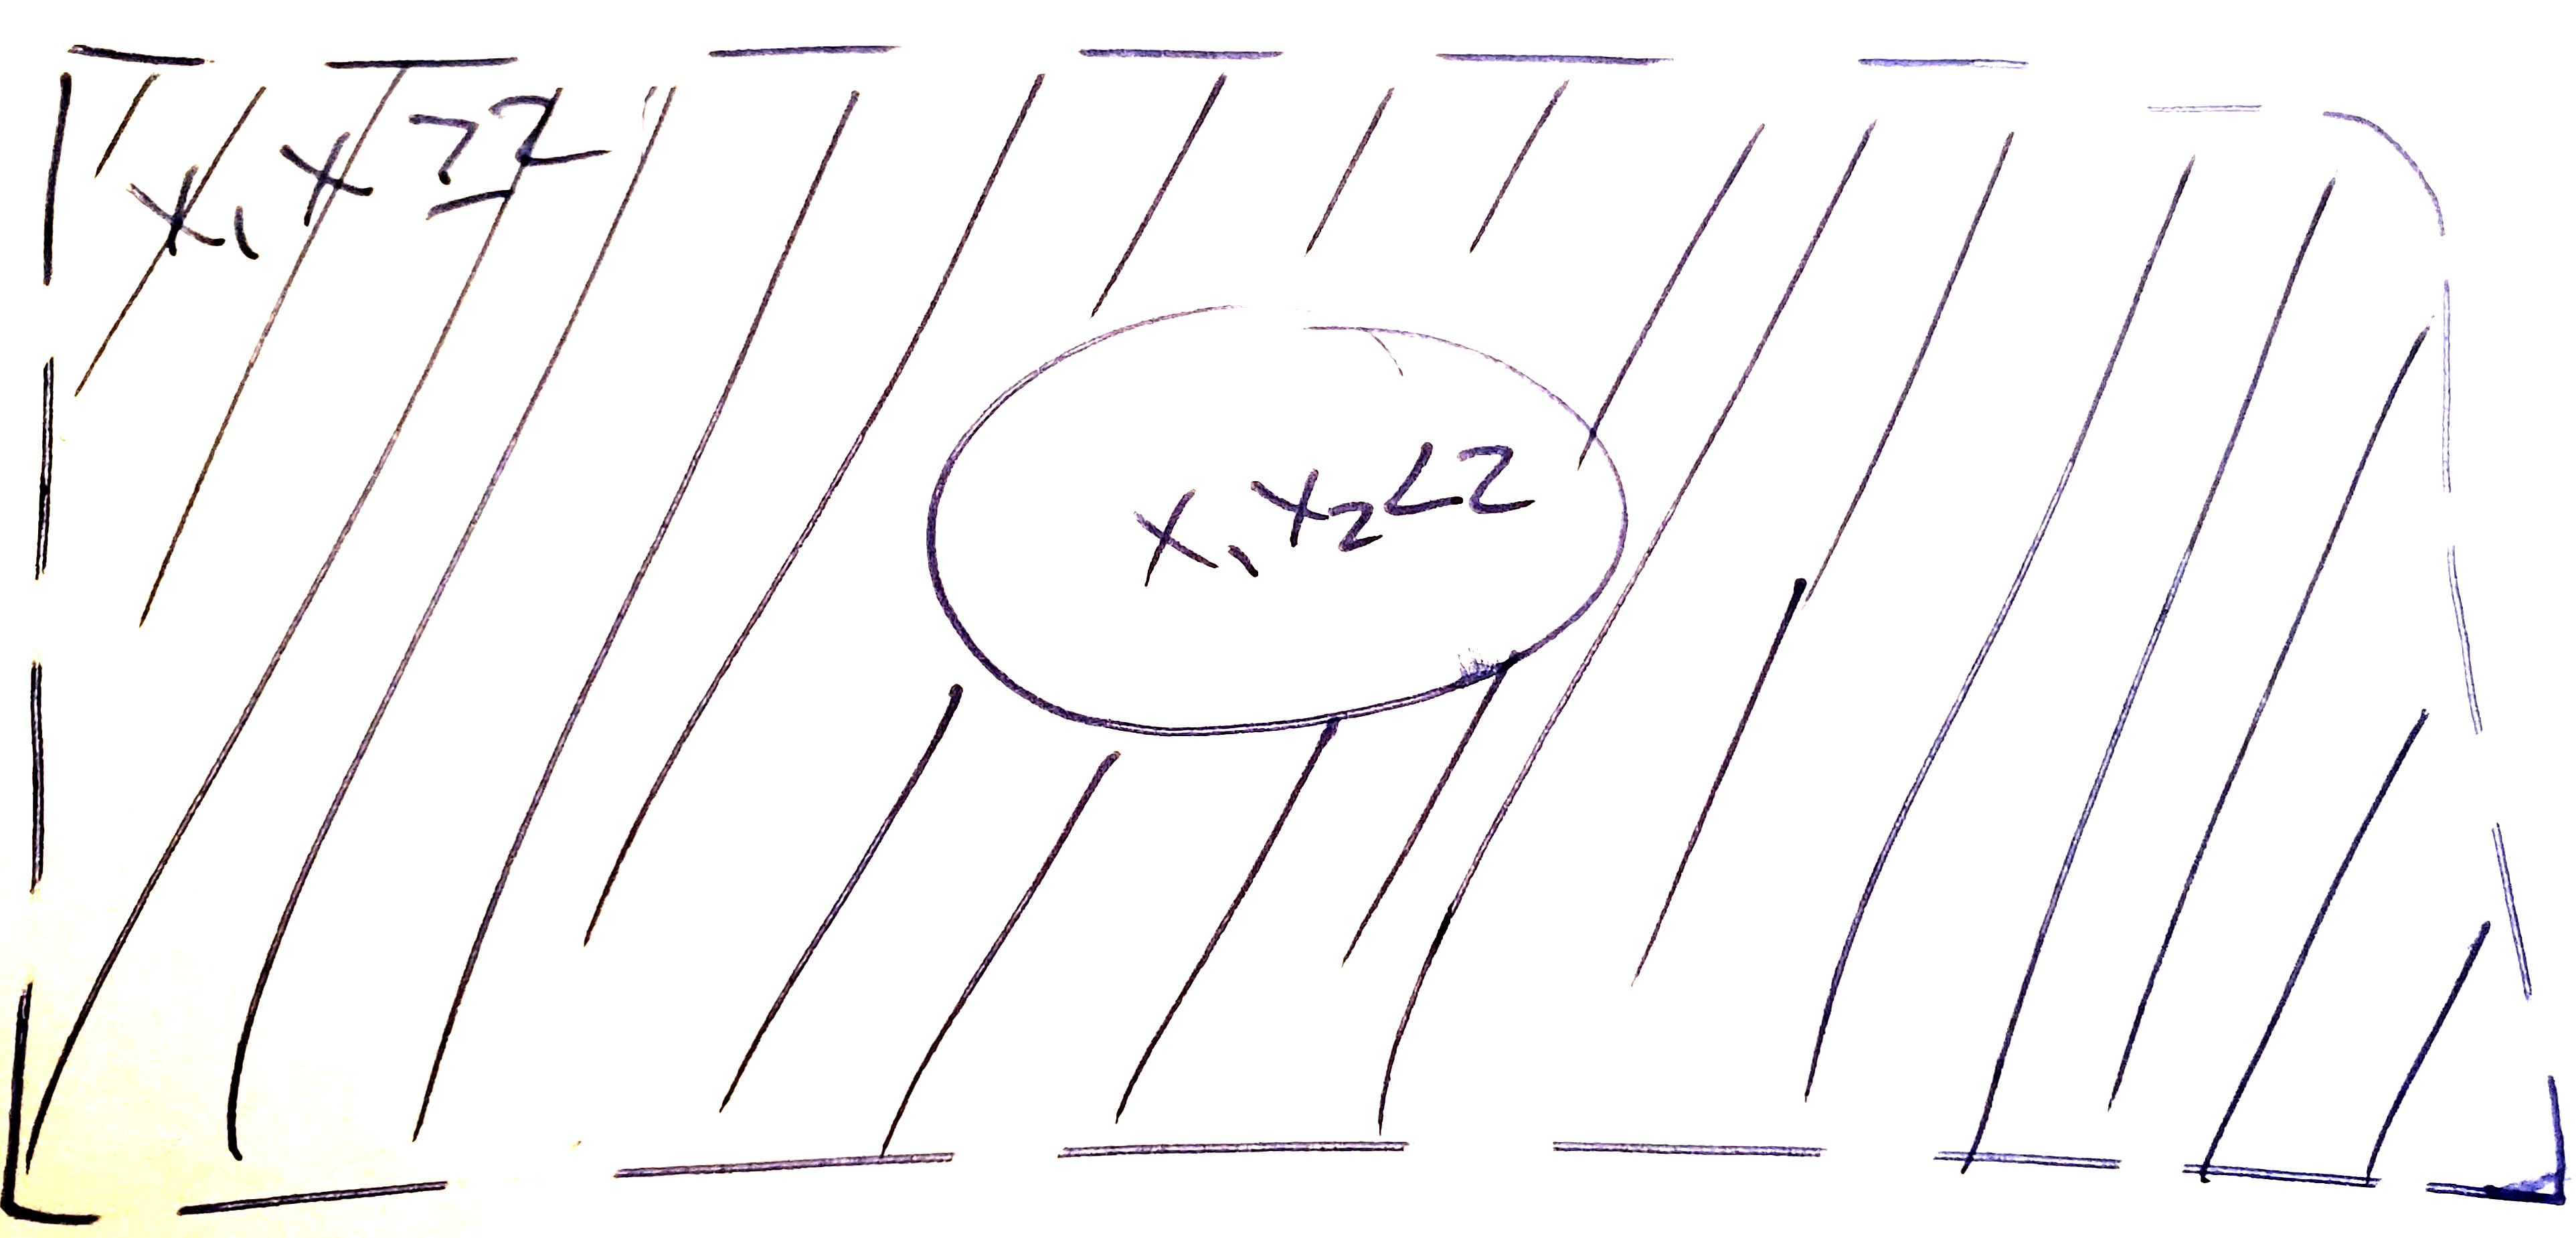
\includegraphics[scale=0.35]{InvariantSet}
\end{center}

\noindent In this picture, we can see that that \underline{positively invariant set $\Gamma$} includes everything except set where $x_1x_2 <2 \quad \forall x \in \R^2$. And that the set $\Gamma$ is an open set since there is no upper limit on it.

\subsection*{Part D}

Using the conclusion from the previous problem, since we have just shown that the system does not converge towards the origin if initialized in set $\Gamma$, the system is \textbf{not} globally asymptotically stable at $x=0$.
